\begin{multicols}{2}

With the complementary strengths of PET and CT scanners assessing tumor margins and guiding surgical interventions is possible. In the case for staging and diagnosing PDAC, PET/CT achieves sensitivity rates of 89–91\% and specificity rates of 70–72\% in detecting PDAC lesions \cite{TG174}.

Key applications include:
\begin{itemize}
	\item \textbf{Tumor Localization and Metastases Detection}: PET/CT excels in identifying primary tumors and distant metastases by FDG concentrated regions lighting up. Zhang et al. demonstrated its utility in detecting rare metastatic sites, such as cutaneous and muscle involvement\cite{Zhang2023}.
	\item \textbf{Lymph Node Evaluation}: In cancer, lymph nodes often act as early sites for metastasis. PET/CT is a great tool to assess lymph node involvement. When FDG concentrates it shows increased glucose metabolism due to cancer activity. This is unique information from PET since lymph nodes may appear normal in size on CT but are metabolically active. Accurate identification of these cancerous nodes improves staging precision, which is critical for planning surgeries, such as lymphadenectomy (removal of affected nodes), and for deciding if curative treatments are feasible \cite{TG174}.
	\item \textbf{Differentiating Lesions}: Since FDG uptake is non-specific, combining metabolic imaging with clinical markers (e.g., IgG4 levels) can help distinguish autoimmune pancreatitis from PDAC \cite{Zheng2018}.
\end{itemize}

Another one of the emerging technologies is the Total Body PET/CT systems. This systems seek to enable whole-body imaging in a single scan, hopefully with enhanced resolution and reduced scanning time \cite{SunderlandSeminar}. This is a valuable innovation for detecting micrometastases and monitoring therapeutic responses. %how is different from normal?

%\section{Applications of [18F]FDG-PET/CT}

PET/CT can be of great help during the different parts of treatment, from diagnosis, staging, to management of pancreatic cancer. In order to exemplify its applications three clinical cases are introduced:

\begin{itemize}
	\item \textbf{Case 1 - Zheng et al.:} 
	A 67-year-old male  with suspected pancreatic cancer presented, in 2018, a metabolic active lesion was identified using a PET/CT scanner. This lesion is located in the head of pancreas and had hinted overlap of metabolic signatures typical of both malignancy and autoimmune pancreatitis\cite{Zheng2018}.
	\item \textbf{Case 2 - Zhang et al.:} 
	In 2023 case, a 64-year-old male with confirmed pancreatic adenocarcinoma and treated with radical resection 6 years earlier presented rare metastatic sites and was reevaluated\cite{Zhang2023}.
	\item \textbf{Case 3 - Deng et al.:} 
	Study in 2021 that compared FDG with 68Ga-FAPI, Gallium-68-labeled Fibroblast Activation Protein Inhibitor, in a 58-year-old female with pancreatic cancer and liver metastases. DG-PET/CT identified hypermetabolic liver lesions, but 68Ga-FAPI demonstrated superior sensitivity in delineating hypodense metastases\cite{Deng2021}.
\end{itemize}

These cases together exemplify applications in the diagnosis and staging of pancreatic cancer of this imaging modality.

\subsection{Tumor Localization and Metabolic Assessment}

\textbf{Metabolic Imaging in Practice:} As stated before the value of FDG-PET resides on the its ability to visualize regions of increased glucose metabolism, even in lesions not that well defined morphologically. A case application is the results of Deng et al. where FDG-PET/CT effectively detects hypermetabolic pancreatic tumors. But, new tracers like 68Ga-FAPI outperform FDG in identifying micrometastases, particularly in hypodense liver lesions \cite{Deng2021}. %differences on the isotope

Figure~\ref{fig:DengMerged} illustrates the comparative uptake of 68Ga-FAPI and 18F-FDG in pancreatic cancer with liver metastases, the maximum density projection (MIP) image (A) shows increased FDG uptake in a pancreatic mass and mild uptake in the 10th rib, suggesting bone metastasis. Axial PET/CT images (B) highlight moderate uptake in the pancreatic head, while (C) reveals minimal bone destruction with mild metabolic activity in the 10th rib. Additionally, small hypodense nodules in the liver (D) were identified without significant FDG uptake, raising suspicion for liver metastases.

\textbf{Quantitative Metrics in Action:} The metric of choice is the Standardized Uptake Value (SUV), it measures FDG uptake in a lesion relative to a reference. The lower the SUV the better as it correlates to malignancy. By knowing this parameter it is posiible to identify micrometastatic lesions, particularly in the liver. Deng et al. shows that 68Ga-FAPI has superior sensitivity highlighting it as a promising area for future research on radiotracers.\cite{Deng2021}

\end{multicols}
% walk thru
\begin{figure}[ht]
	\centering
	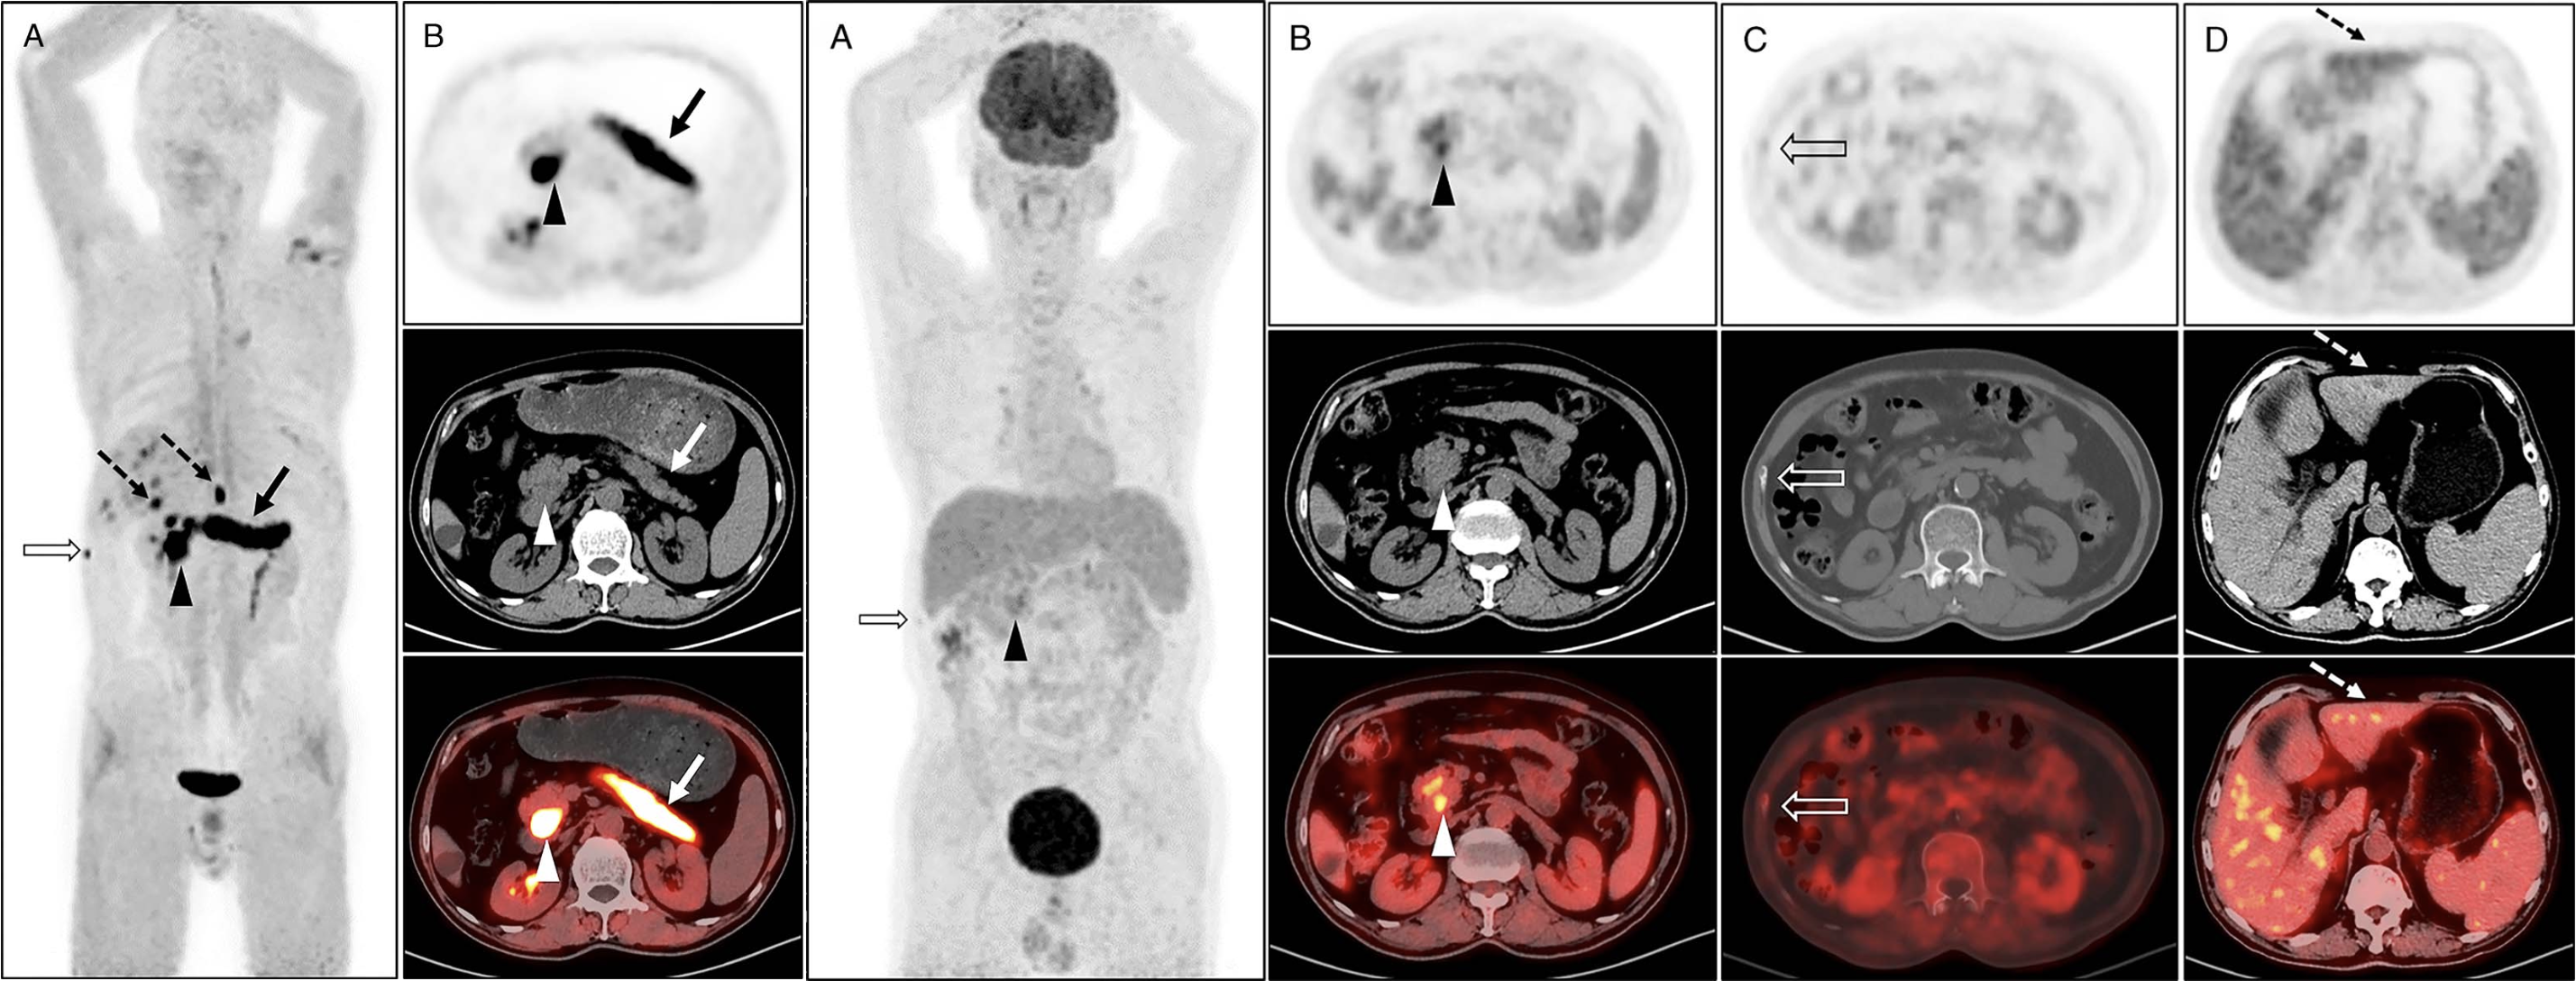
\includegraphics[width=0.9\textwidth]{assets/DengMerged.png}
	\caption{Comparison of FDG-PET/CT metabolic activity. (Right) 18F-FDG PET/CT showing pancreatic mass and liver hypodense lesions with minimal uptake, highlighting its sensitivity in tumor and liver staging \cite{Deng2021}. (Left) Enhanced metabolic activity in pancreatic lesions with high resolution, 68Ga-FAPI tracer’s specificity in hypometabolic areas near liver\cite{Deng2021}.}
	\label{fig:DengMerged}
\end{figure}


%---


\begin{multicols}{2}
\subsection{Lymph Node Evaluation and Metastasis Detection}

\textbf{Unique Metastases:} 
In case 2, PET/CT demostrated its capacity to distiguish between muscle and cutaneous metastases from PDAC—locations rarely detected by conventional imaging. Without PET/CT this would be possible to asses correctly

Figure~\ref{fig:Zhang1}, depicts a MIP image with two regions of elevated glucose metabolism (Upper abdomen and left lateral abdominal wall). An axial image of the anatomy shows near the surgery site that shows elevated metabolic activity, possibly indicating residual or recurrent cancer, or post-surgical inflammatory changes. Then focused on the lateral it shows an hypodense structure seen in the muscle. This is the rare case of a metastatic deposit in the muscle. They highlight that Muscle metastases from pancreatic cancer are exceptionally rare, while cutaneous metastases occur in only 0.5–7.6\% of cases, often at the umbilicus\cite{Zhang2023}.


\textbf{Sensitivity and Specificity:} Zhang et al. found that FDG uptake reliably identifies malignancies, it may also highlight non-malignant inflammatory processes, necessitating careful interpretation and, when possible, the inclusion of additional clinical markers or advanced tracers.


\end{multicols}

\begin{figure}[H]
	\centering
	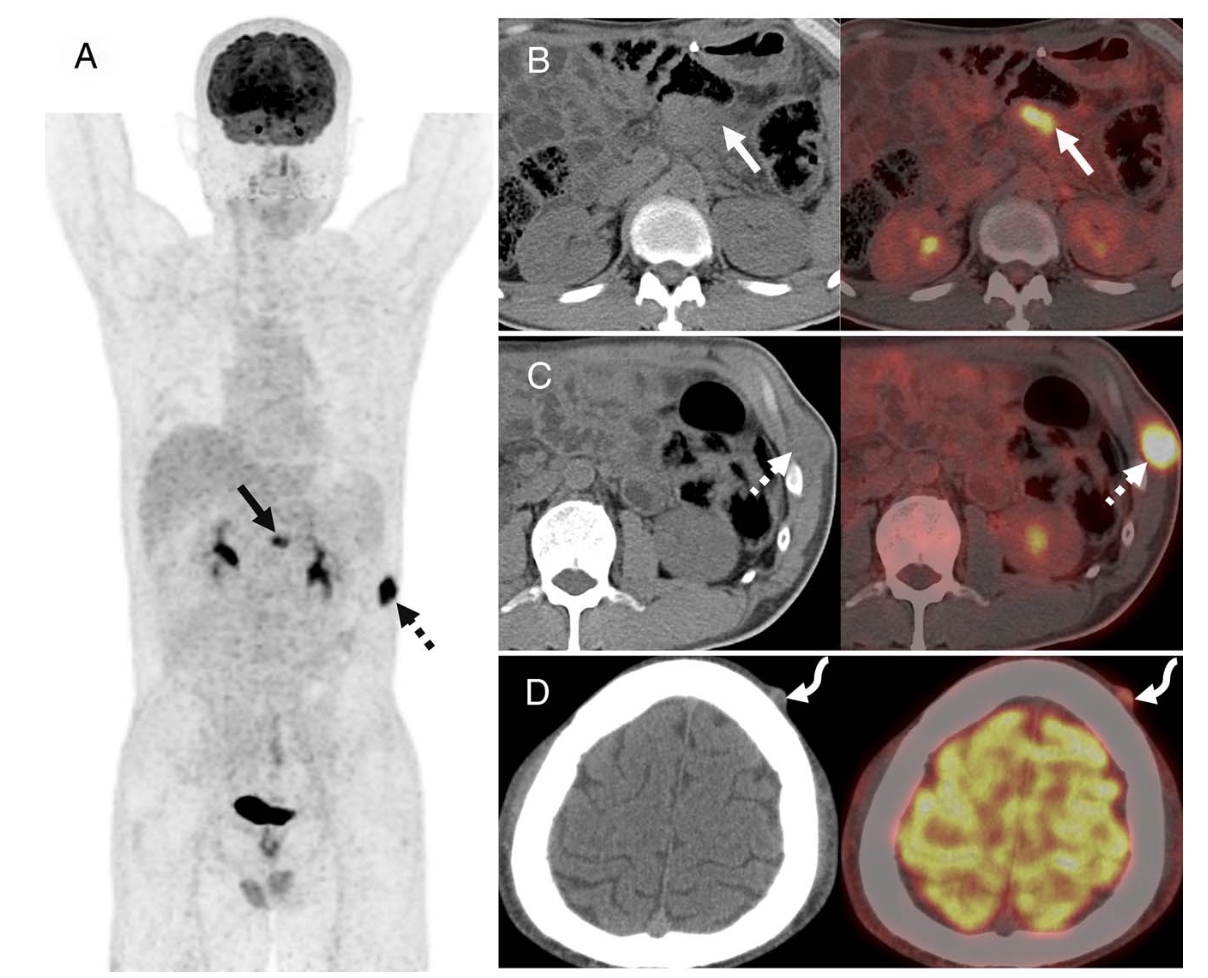
\includegraphics[width=0.75\textwidth]{assets/Zhang1.png}
	\caption{Rare cutaneous and muscle metastases detected using FDG-PET/CT, illustrating its capability for identifying uncommon metastatic sites \cite{Zhang2023}.}
	\label{fig:Zhang1}
\end{figure}

%---

\subsection{Treatment Planning and Monitoring}

\textbf{Guiding Therapy with PET/CT:} In order to perform a surgical resection and radiation therapy the boundaries of the tumor must be carfully delinated. Zheng et al. were able to differentiate autoimmune pancreatitis from PDAC from this images, avoiding unnecessary or ineffective treatments \cite{Zheng2018}.

%explain figures
Figure~\ref{fig:Zheng1} showcases how PET/CT identifies metabolic distinctions that inform treatment in challenging cases where inflammatory and malignant lesions overlap. Additionally, post-treatment PET/CT imaging provides insights into metabolic response, that enables clinicians to adjust therapeutic regimens based on observed changes in FDG uptake.

\textbf{Enhancing Planning with Alternative Tracers:} As noted in Deng et al., the integration of new tracers like 68Ga-FAPI offers improved sensitivity in hypoxic tumor regions. \cite{Deng2021}.

\begin{figure}[H]
	\centering
	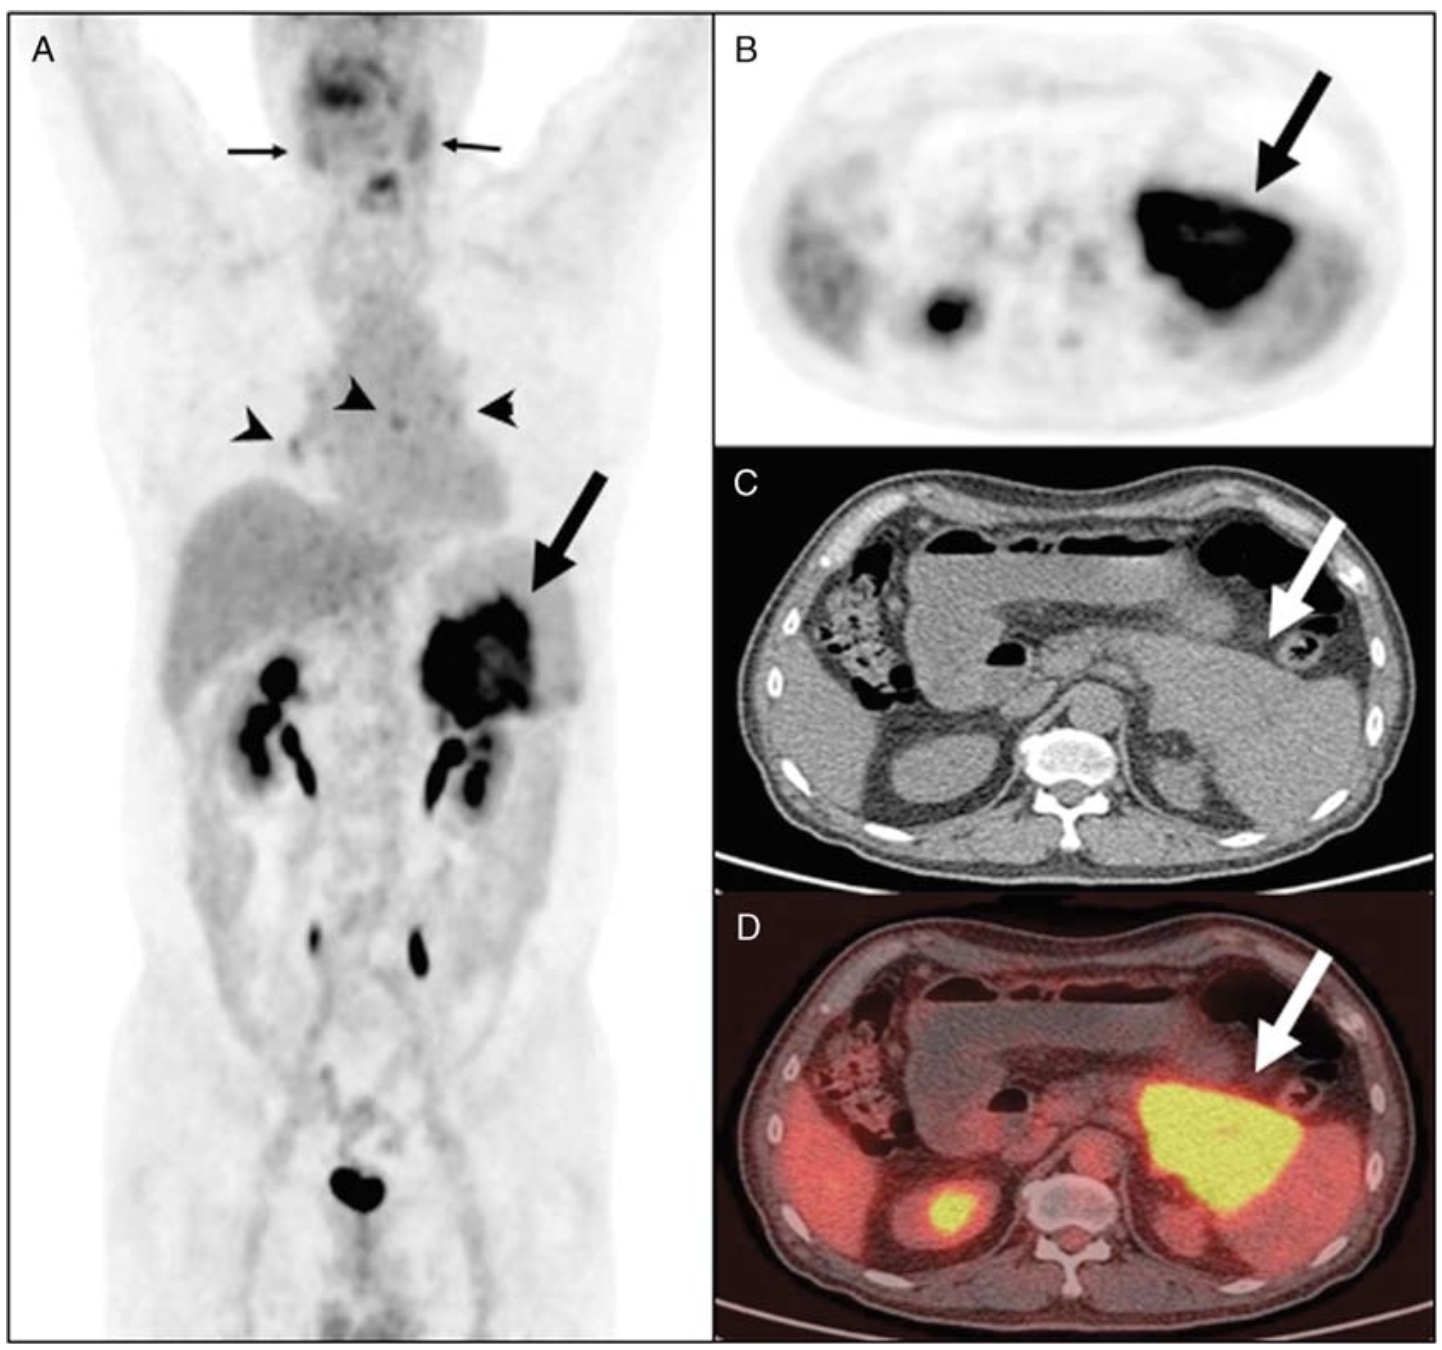
\includegraphics[width=0.75\textwidth]{assets/Zheng1.png}
	\caption{FDG-PET/CT imaging showing focal autoimmune pancreatitis mimicking pancreatic cancer. Note: the overlapping metabolic activity that challenges differentiation \cite{Zheng2018}.}
	\label{fig:Zheng1}
\end{figure}

%---

Section 4 demonstrated the utility that PET/CT provides to diagnosis, staging, and management of pancreatic cancer. These clinical cases are an example of the current technology and limitations that we have in terms of resolution and specificity, and accessibility. Addressing these limitations will lean this technology forward for better and precise treatment, innovations in radiotracer development and hybrid imaging modalities can certainly be the way forward.
